%Copyright 2019 Christopher M. Jermaine (cmj4@rice.edu) and Risa B. Myers (rbm2@rice.edu)
%
%Licensed under the Apache License, Version 2.0 (the "License");
%you may not use this file except in compliance with the License.
%You may obtain a copy of the License at
%
%    https://www.apache.org/licenses/LICENSE-2.0
%
%Unless required by applicable law or agreed to in writing, software
%distributed under the License is distributed on an "AS IS" BASIS,
%WITHOUT WARRANTIES OR CONDITIONS OF ANY KIND, either express or implied.
%See the License for the specific language governing permissions and
%limitations under the License.
%===============================================================
\documentclass[aspectratio=169]{beamer}
\mode<presentation> 
{
\usetheme[noshadow, minimal,numbers,riceb,nonav]{Rice}
\usefonttheme[onlymath]{serif}
\setbeamercovered{transparent}
}
\useinnertheme{rectangles}
\usepackage{multirow}

\usepackage[english]{babel}

\usepackage{mathptmx}
\usepackage{helvet}
\usepackage{courier}
\usepackage[T1]{fontenc}
\usepackage{trajan}
\usepackage{ textcomp }
\usepackage{listings}

\newenvironment{noindentitemize}
{ \begin{itemize}
 \setlength{\itemsep}{1.5ex}
  \setlength{\parsep}{0pt}   
  \setlength{\parskip}{0pt}
 \addtolength{\leftskip}{-2em}
 }
{ \end{itemize} }

\newenvironment{noindentitemize2}
{ \begin{itemize}
  \setlength{\itemsep}{0ex}
  \setlength{\parskip}{0pt}
  \setlength{\parsep}{0pt}   
  \addtolength{\leftskip}{-2em}  }
{ \end{itemize} }



\lstnewenvironment{SQL}
  {\lstset{
        aboveskip=5pt,
        belowskip=5pt,
        escapechar=!,
        mathescape=true,
        upquote=true,
        language=SQL,
        basicstyle=\linespread{0.94}\ttfamily\footnotesize,
        morekeywords={PRINT, CURSOR, OPEN, FETCH, CLOSE, DECLARE, BEGIN, END, PROCEDURE, FOR, EACH, WITH, PARTITION, 	TEST, WHETHER, PROBABILITY, OUT,LOOP,IF,CONTINUE, HANDLER,CALL, FUNCTION, RETURNS, LANGUAGE,BODY,RETURN, REPLACE,plpgsql,
        RAISE, NOTICE,
        REPLACE, ROW, BEFORE, EXIT, TEXT, REFCURSOR, QUOTE_LITERAL, DELIMITER,CONCAT,FOUND,LEAVE },
        deletekeywords={VALUE, PRIOR},
        showstringspaces=true}
        \vspace{0pt}%
        \noindent\minipage{0.65\textwidth}}
  {\endminipage\vspace{0pt}}
  
  
\lstnewenvironment{SQLtiny}
  {\lstset{
        aboveskip=5pt,
        belowskip=5pt,
        escapechar=!,
        mathescape=true,
        upquote=true,
        language=SQL,
        basicstyle=\linespread{0.94}\ttfamily\tiny,
        morekeywords={PRINT, CURSOR, OPEN, FETCH, CLOSE, DECLARE, BEGIN, END, PROCEDURE, FOR, EACH, WITH, PARTITION, 	TEST, WHETHER, PROBABILITY, OUT,LOOP,IF,CONTINUE, HANDLER,CALL, FUNCTION, RETURNS, LANGUAGE,BODY,RETURN, REPLACE,plpgsql,
        RAISE, NOTICE,
        REPLACE, ROW, BEFORE, EXIT, TEXT, REFCURSOR, QUOTE_LITERAL, DELIMITER,CONCAT,FOUND,LEAVE },
       deletekeywords={VALUE, PRIOR},
        showstringspaces=true}
        \vspace{0pt}%
        \noindent\minipage{0.47\textwidth}}
  {\endminipage\vspace{0pt}}

%===============================================================%

\title[]
{Tools \& Models for Data Science}

\subtitle{Linear Regression}

\author[]{Chris Jermaine \& Risa Myers}
\institute
{
  Rice University 
}

\date[]{}

\subject{Beamer}


\begin{document}
%***********************************************************

\begin{frame}
 \titlepage
\end{frame}
%***********************************************************

\begin{frame}{Linear Regression}

\begin{columns}
\begin{column}{0.5\textwidth}
\begin{itemize}
	\item Most common model in data science! (Logistic Regression is very common as well)
	\begin{itemize}
		\item Have a set of training data
		\item Bunch of $(x_i, y_i)$ pairs
		\item $x_i$ is a vector of real-valued ``regressors'' / features / dimension
		\item $y_i$ is a real-valued ``response''
		\item Want to learn a model that, given a new $x$, can predict $y$
	\end{itemize}
\end{itemize}
 \end{column}
\begin{column}{0.5\textwidth}
     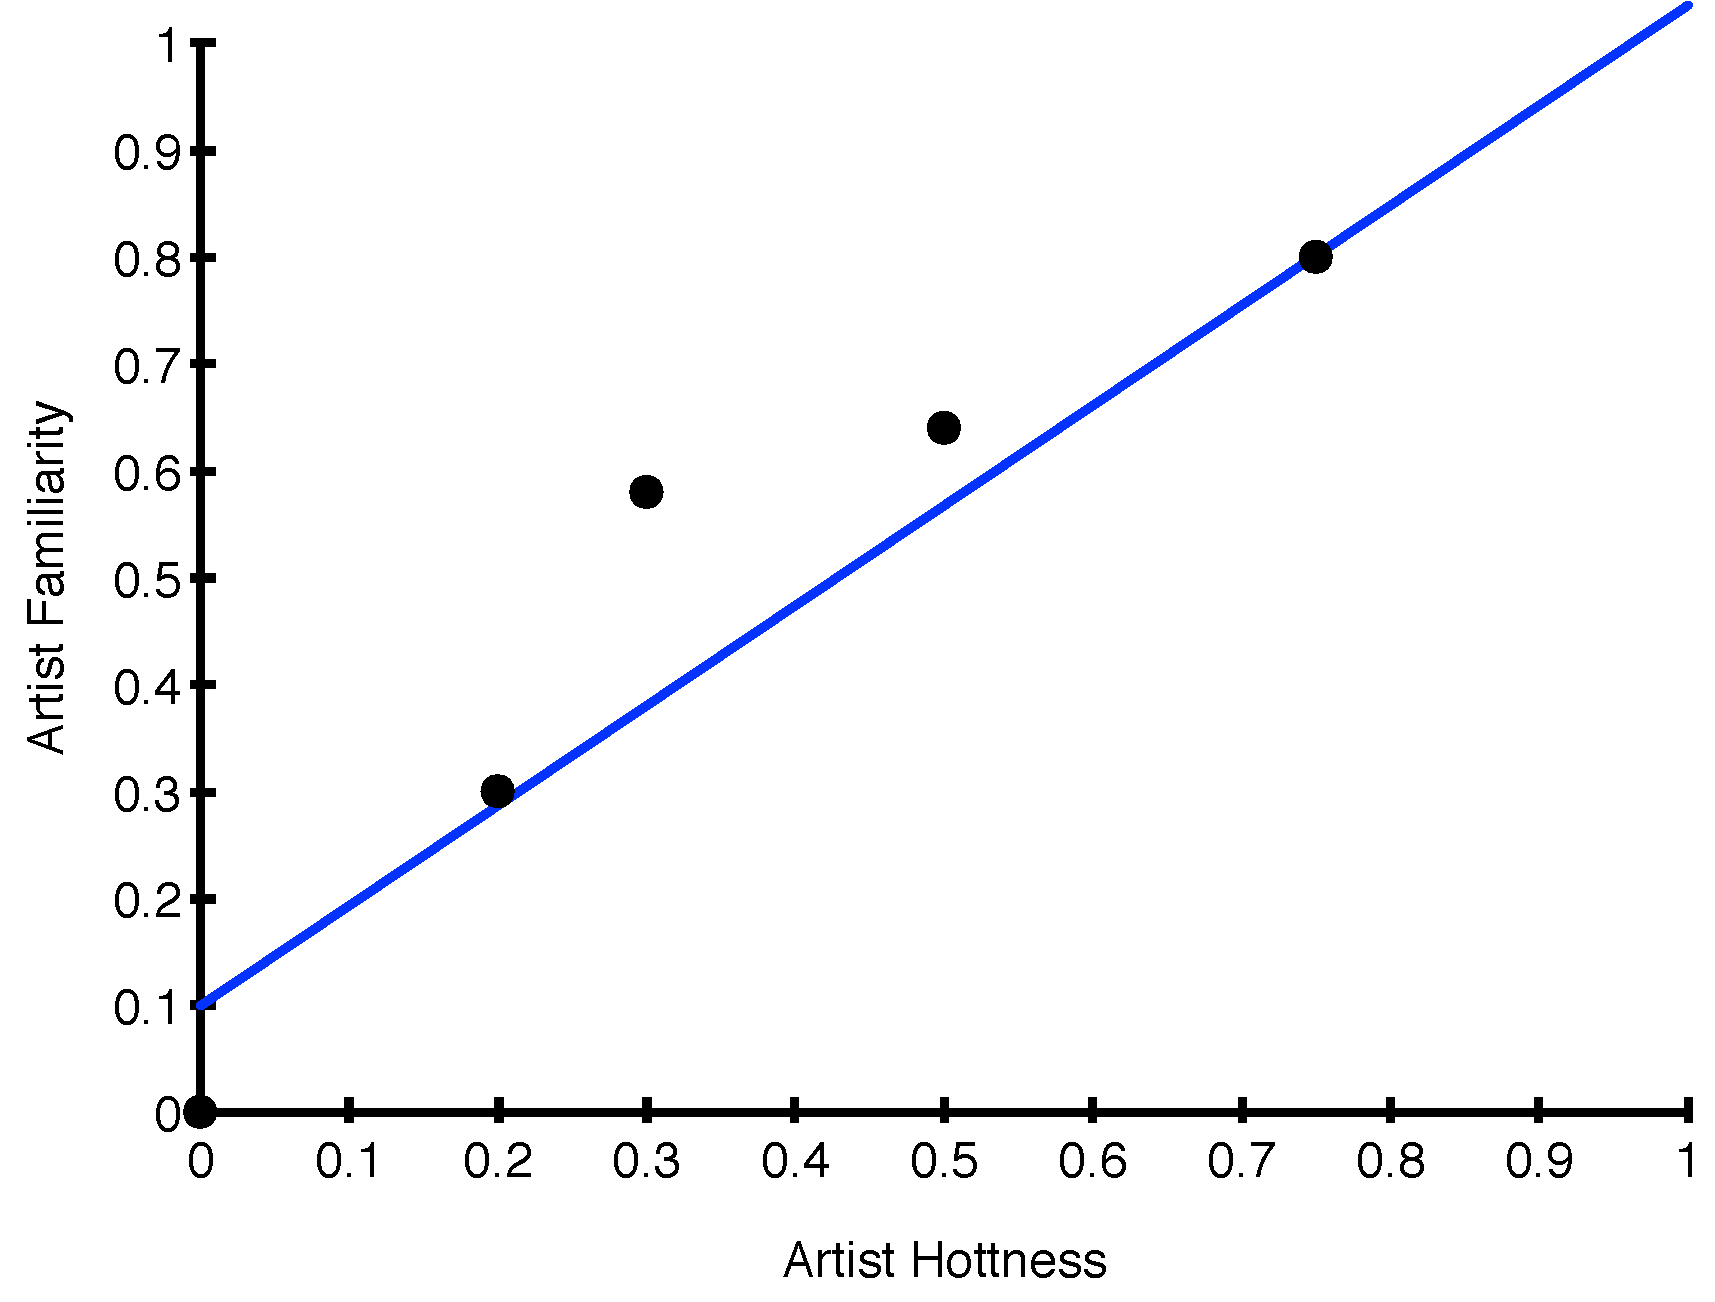
\includegraphics[width=1\textwidth]{lectLR/hotVsFam.pdf} 
\end{column}
 \end{columns}

\end{frame}
%***********************************************************
\begin{frame}{Linear Regression}

\begin{itemize}
	\item Model is exceedingly simple
	\begin{itemize}
		\item Predict $\hat{y}$ as $x \cdot r$
		\item $r$ is a vector of ``regression coefficients'' 
		\item $x \cdot r$ is the dot product of: $x \cdot r = \sum_j x_j \times r_j = \hat{y_i}$
		\item Can be used with loss functions:
		\begin {itemize}
			\item  Least Squares (L2 norm)  
			$$Loss = \lVert y - f(x)\rVert^2_2$$
			\item Mean Squared Error (MSE), where $n$ is the number of training points
			$$Loss =\frac{ \lVert y - f(x)\rVert^2_2}{n}$$
			\item Others...
		\end{itemize}
	\end{itemize}
\end{itemize}
\end{frame}

%***********************************************************
\begin{frame}{Regression Coefficient Example}

\begin{columns}
\begin{column}{0.5\textwidth}
\begin{itemize}
	\item Specify the weight/importance and direction of each feature
	\item Weight is indicated with magnitude
	\item Direction is indicated by the sign
\end{itemize}
\end{column}
\begin{column}{0.5\textwidth}
Predicting Song Tempo
\begin{tabular}{|l|r|}\hline
& \textbf{Regression } \\ 
& \textbf{ Coefficient } \\ 
\textbf{Feature} & \textbf{value} \\ \hline
Duration       &     -0.0061 \\ \hline
Latitude      &     -0.1197\\ \hline
Loudness          &  1.1527\\  \hline
Year          &  0.0013\\  \hline
Intercept   &     139.72\\  \hline
\end{tabular}
\end{column}
\end{columns}
\end{frame}
%***********************************************************
\begin{frame}{Our Data}

\begin{itemize}
		\item Let the matrix $\textbf{X}$ store the training data
		\item $i$th row in $\textbf{X}$ is $i$th training point, $x_i$
		\item $\textbf{y}$ is a column vector storing responses\
\[
 \textbf{X}  = \begin{bmatrix} 
 \rule[.025in]{1in}{0.5pt}	&x_1  & \rule[.025in]{1in}{0.5pt}	\\
 \rule[.025in]{1in}{0.5pt}	&x_2  & \rule[.025in]{1in}{0.5pt}	\\
	& $\vdots$ & 	\\
\rule[.025in]{1in}{0.5pt}		&x_i & \rule[.025in]{1in}{0.5pt}		\\
	&$\vdots$  & 	\\
 \rule[.025in]{1in}{0.5pt}	&x_n  & \rule[.025in]{1in}{0.5pt}	\\
\end{bmatrix} 
\textbf{y} = \begin{bmatrix} 
	 & y_1  & 	\\
	 & y_2  & 	\\
	 &  $\vdots$ & 	\\
	 & y_i & 	\\
	 & $\vdots$ & 	\\
	 & y_n& 	\\
\end{bmatrix} 
\]

 \end{itemize}
\end{frame}
%***********************************************************
\begin{frame}{How to Learn?}

\begin{itemize}
	\item Turns out there is a closed-form solution to this minimization problem we are solving for regression
        \begin{itemize} 
%		\item Let the matrix $\textbf{X}$ store the training data
%		\item $i$th row in $\textbf{X}$ is $i$th training point, $x_i$
%		\item $\textbf{y}$ is column vector storing responses
		\item Then closed form least-squares estimate for $r$ is (you can look this up):
			$$\hat{r} = (\textbf{X}^{\textrm{T}}\textbf{X})^{-1}\textbf{X}^{\textrm{T}}\textbf{y}$$
		\item This minimizes loss:
%			$$ \sum_i (y_i - \sum_j x_{i,j} \times r_j)^2$$
			$$ \sum_i (y_i - x_i \times r)^2$$
	\end{itemize}
\end{itemize}
\end{frame}
%***********************************************************
\begin{frame}{Problematic for ``Big Data''}

\begin{itemize}
	\item[] 			$$\hat{r} = (\textbf{X}^{\textrm{T}}\textbf{X})^{-1}\textbf{X}^{\textrm{T}}\textbf{y}$$
	\item But this can be problematic for ``Big Data''... why?
\end{itemize}
\end{frame}
%***********************************************************
\begin{frame}{Problematic for ``Big Data''}

\begin{itemize}
		\item Matrix may be too big to fit in memory
		\item e.g. 1 dataset of 1 Billion observations / data points
		%\item 1K dimensions = 8 Tb of memory
		\vspace{5em}
		\item So, how can we perform linear regression on big data?
\end{itemize}
\end{frame}
%***********************************************************
\begin{frame}{More Reasonable Big Data Formulation}

\begin{itemize}
\item Recall the closed form least squares estimator for $\hat{r}$:
			$$\hat{r} = (\textbf{X}^{\textrm{T}}\textbf{X})^{-1}\textbf{X}^{\textrm{T}}\textbf{y}$$
	\item We can compute $(\textbf{X}^{\textrm{T}}\textbf{X})^{-1}$ as:
		$$\left( \sum_i x_i^{\textrm{T}} x_i \right)^{-1}$$
		\begin{itemize}
			\item Note: assumes $x_i$ is a row vector
			\item $ x_i^{\textrm{T}} x_i $ is the outer product of $x_i$ with itself, resulting in an $n\times n$ matrix
			\item Recall from lab that $x_i^{\textrm{T}} x_i$ is the sum of the outer products of the matrix rows
		\end{itemize}
	\item[?] What's great about this formulation?
\end{itemize}
\end{frame}
%***********************************************************
\begin{frame}{More Reasonable Big Data Formulation (continued)}

\begin{itemize}
	\item Compute $(\textbf{X}^{\textrm{T}}\textbf{X})^{-1}$ as:
		$$\left( \sum_i x_i^{\textrm{T}} x_i \right)^{-1}$$
	\item What's great about this formulation?
\begin{itemize}
	\item It can be parallelized!
	\item Distribute blocks  of rows (say 100) at a time
	\item Compute the products
	\item Collect,  reassemble, sum, then invert
\end{itemize}
\end{itemize}
\end{frame}

%***********************************************************
\begin{frame}{More Reasonable Big Data Formulation (continued)}

\begin{itemize}
	\item Goal: Compute the closed form least squares estimate for $\hat{r}$
			$$\hat{r} = (\textbf{X}^{\textrm{T}}\textbf{X})^{-1}\textbf{X}^{\textrm{T}}\textbf{y}$$
\begin{enumerate}
	\item Compute $(\textbf{X}^{\textrm{T}}\textbf{X})^{-1}$ as (per the last slide):
		$$\left( \sum_i x_i^{\textrm{T}} x_i \right)^{-1}$$
	\item Compute $\textbf{X}^{\textrm{T}}\textbf{y}$ as:
		$$\left( \sum_i (x_i \times y_i) \right)^{\textrm{T}}$$
\end{enumerate}
\item \#2 can also be parallelized
\item since it is a sum of products
\end{itemize}
\end{frame}
%***********************************************************
\begin{frame}{Still, Bad for Very High-D Data}

\begin{itemize}
	\item[] 	$$\left( \sum_i x_i^{\textrm{T}} x_i \right)^{-1} \left( \sum_i (x_i \times y_i) \right)^{\textrm{T}}$$

        \item[?] Why?
\end{itemize}

\end{frame}
%***********************************************************
\begin{frame}{Problematic for Very High-D Data}

\begin{itemize}
	\item Inverting $\textbf{X}$ can be expensive, if the number of dimensions is high
	\begin{itemize}
		\item $\approx$ 100K $\times$ 100K is an upper limit for a single machine
		\item Laptop maxes out at 4-8K $\times$ 4-8K
		\item The matrix doesn't fit in memory!
		%\item Easily get to this size with 4-grams in text % we didn't cover these yet
	\end{itemize}
	\vspace{2em}
	\item[?] What's the solution?
\end{itemize}
\end{frame}
%***********************************************************
\begin{frame}{Problematic for Very High-D Data}

\begin{itemize}
	\item Closed form LR takes too much memory for High-D data
	\item So, don't use it!
	\item Instead, use Gradient Descent on the Mean Squared Error Loss function:
	$$\frac{\sum_i(y_i - x_i \times r)^2}{n}$$
	\item where $r$ is the vector of regression coefficients
	\item and $n$ is the number of data points
\end{itemize}
\end{frame}
%***********************************************************
\begin{frame}{Gradient Descent on MSE}

\begin{itemize}
	\item The partial derivative of the loss function wrt $r_j$ is:
	$$\frac{\partial}{\partial r_j}\frac{ \sum_i (y_i - \sum_{j'} x_{i,j'} \times r_{j'})^2}{n} = \frac{\sum_i -2(y_i - \hat{y}_i) x_{i,j}}{n}$$
	\item Where $\hat{y}_i$ is the prediction for $y_i$ given the current model
	\item Again, this expression can be parallelized 
\end{itemize}

\end{frame}
%***********************************************************
\begin{frame}[fragile]{Gradient Descent Algorithm}
\begin{SQL}
$n \leftarrow \textrm{the number of training data points}$
$r^0 \leftarrow \textrm{non-stupid guess for } r$;
$iter \leftarrow 1$;
repeat {
  for each $j$
    $\Delta_j \leftarrow \sum_i -\frac{2}{n}(y_i - \hat{y}_i) x_{i,j}$
  $r^{iter + 1} \leftarrow r^{iter} - \lambda \Delta$;
  $iter \leftarrow iter + 1$;
} while (change in loss $> \epsilon$)
\end{SQL}

\begin{itemize}
	\item Where $r$ is the vector of regression coefficients
	\item and $n$ is the number of training data points

	\item Say our estimate ($\hat{y}_i$) for point $i$ is too large
        \item That is, $y_i - \hat{y}_i$ is negative (example, $-0.05$)
        \item If $x_{i,j}$ is positive (ex: $2.0$), point $i$ will try to pull $\Delta_j$ so it is positive:
               contribution to $\Delta_j$ is $-\frac{2}{n}(-0.05)2.0 = 0.2$
        \item Since $r^{iter + 1} \leftarrow r^{iter} - \lambda \Delta$, point $i$ will try to decrease $r_j$:
               will contribute a decrease of $\lambda 0.2$
        \item So point $i$ will want the regression coefficient to decrease, which makes sense
\end{itemize}
\end{frame}
%***********************************************************
\begin{frame}{}
\begin{columns}
\begin{column}{0.5\textwidth}
    \end{column}
\begin{column}{0.5\textwidth}
     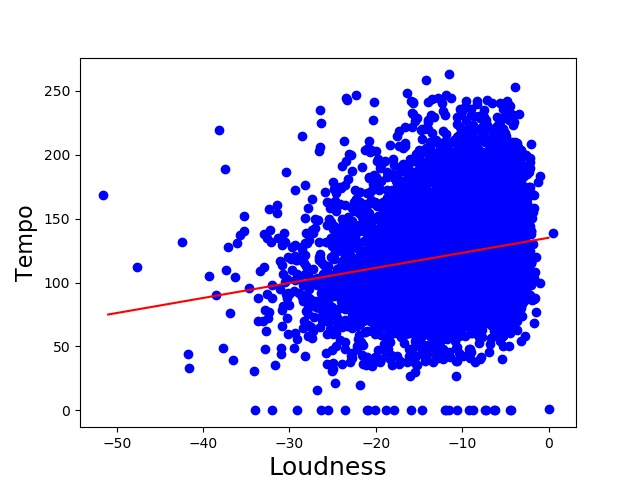
\includegraphics[width=1\textwidth]{lectLR/musicLoudTempo.jpg} 
\end{column}
 \end{columns}

\end{frame}
%***********************************************************
\begin{frame}{Why is this a Good Big Data Algorithm?}

\begin{itemize}
\item[] $$\frac{\partial}{\partial r_j}\frac{ \sum_i (y_i - \sum_{j'} x_{i,j'} \times r_{j'})^2}{n} = \frac{\sum_i -2(y_i - \hat{y}_i) x_{i,j}}{n}$$
\item It's linear in number of data points
\item Also linear in number of regressors (features / dimensions)
\end{itemize}
\end{frame}
%***********************************************************
\begin{frame}{Why is this a Good Big Data Algorithm?}

\begin{itemize}
\item In particular, nice for sparse data (common in really high dimensions)
	\begin{itemize}
	\item If $x_{i,j}$ is zero, no contribution to $\Delta_j$
	\item Note: You must use a sparse matrix representation to benefit
	\end{itemize}
\end{itemize}
\[
%\begin{bmatrix} 
%	 &   & 	\\
%	 &   & 	\\
%	 &   & 	\\
%	 &   & 	\\
%	 & \textbf{X}' & 	\\
%	 &  & 	\\
%	 &  & 	\\
%	 & & 	\\
%\end{bmatrix} 
\textrm{Dense:}
 \begin{bmatrix} 
	0&2 &0& 0	\\
	0&0 &7& 0	\\
	0&0 &0& 0	\\
	4&0 &0& 0	\\
	0&0 &0& 0	\\
	0&0 &0& 1	\\
	0&0 &-5 & 3	\\
\end{bmatrix} 
\textrm{Sparse:}
 \begin{bmatrix} 
	0:& (1,2)	\\
	1:& (2,7)	\\
	2:&	\\
	3:&(0,4)	\\
	4: &	\\
	5:&(3,1)	\\
	6:&(2, -5), (3, 3)	\\
\end{bmatrix} 
\]
\end{frame}
%***********************************************************
\begin{frame}{Why is this a Bad Big Data Algorithm?}

\begin{itemize}
\item It's linear in number of data points
\item Also linear in number of regressors (features / dimensions)
\item Alternatives
\begin{itemize}
\item Mini-batch Gradient Descent - use a small number of randomly sampled data points at each iteration
\item Stochastic Gradient Descent - use a single randomly sampled data point at each iteration
\end{itemize}
\end{itemize}
\end{frame}
%***********************************************************
\begin{frame}{How To Add an Intercept?}

\begin{columns}
\begin{column}{0.5\textwidth}
\begin{itemize}
\item Add an extra column to each data point
\item Always has a ``1'' value
\item[?] Why will this work?
\end{itemize}
\end{column}
\begin{column}{0.5\textwidth}
     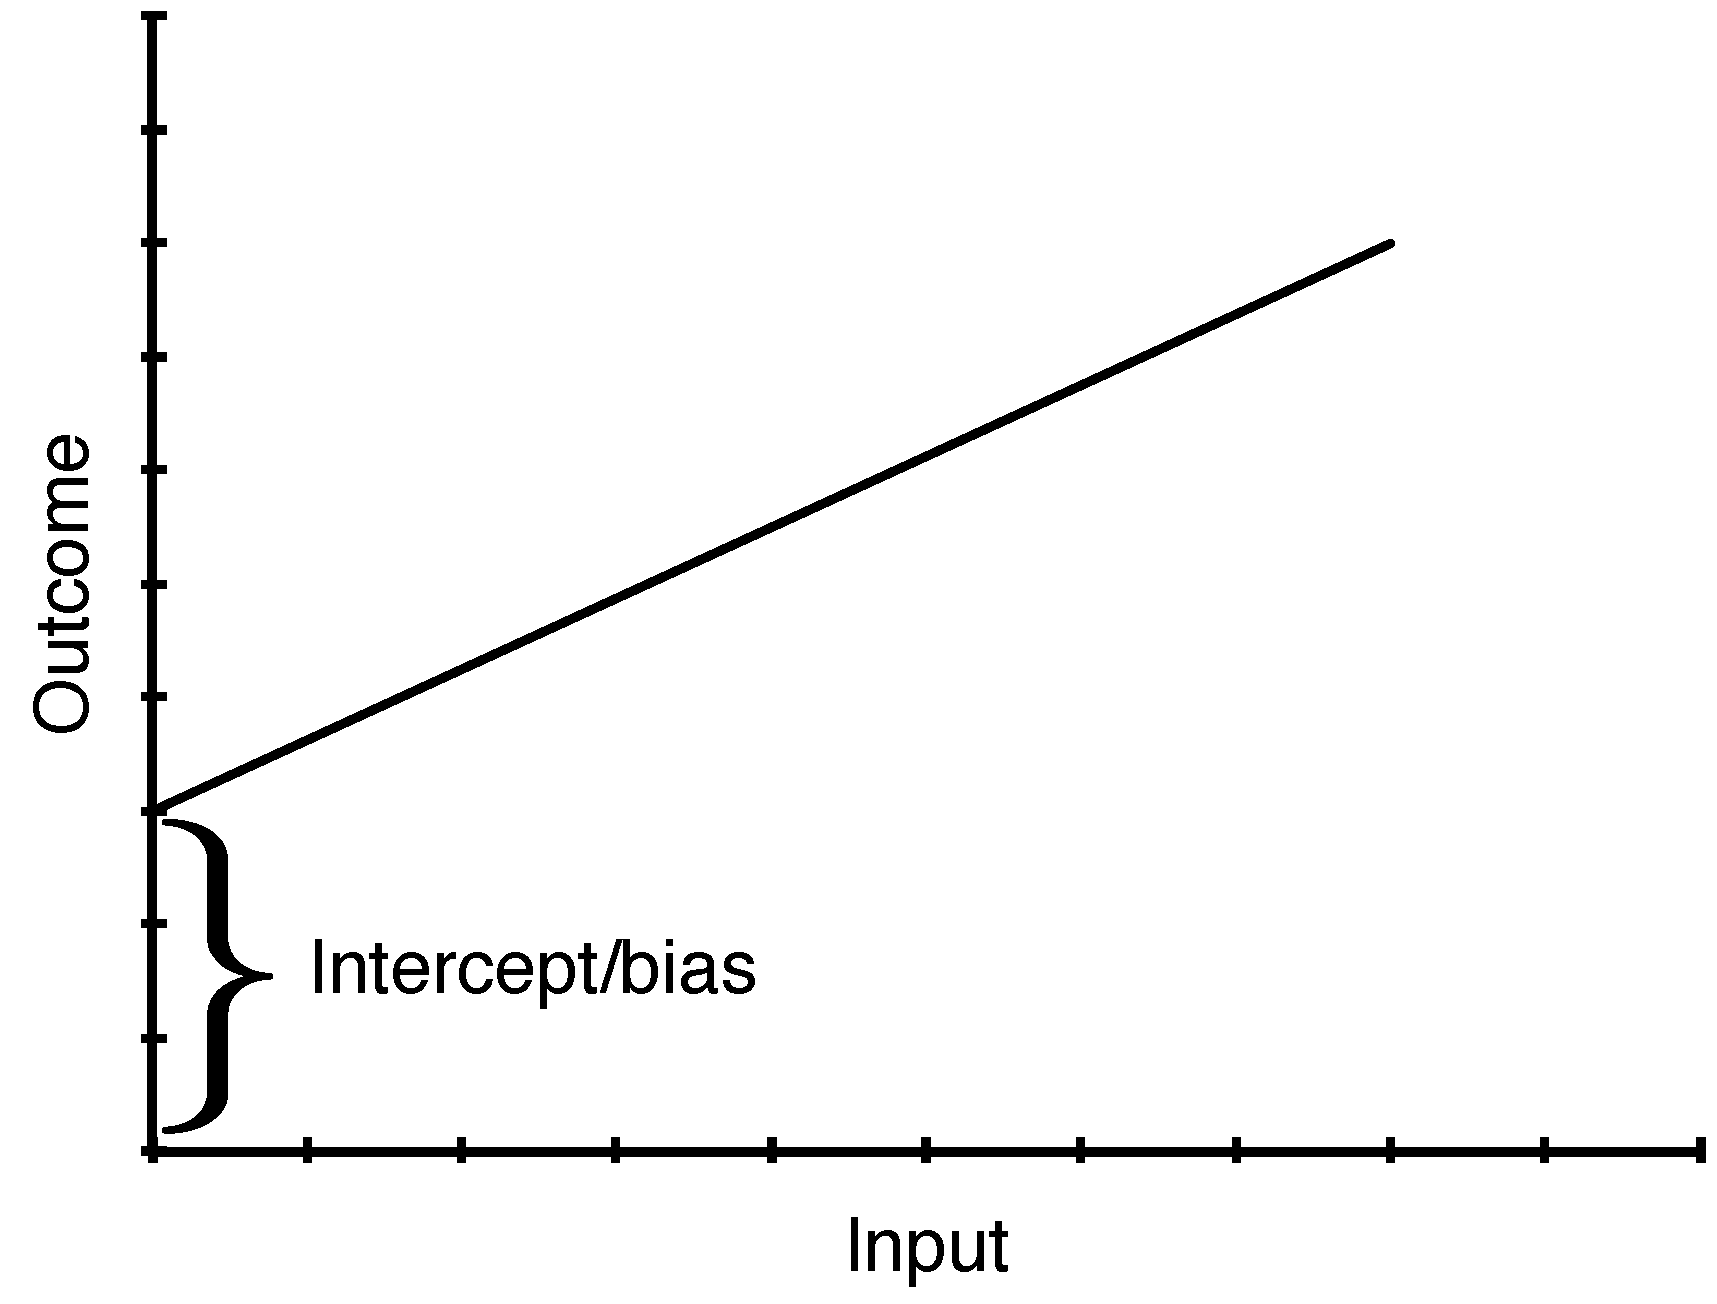
\includegraphics[width=1\textwidth]{lectLR/intercept.pdf} 
\end{column}
\end{columns}
\end{frame}
%***********************************************************
\begin{frame}{How To Add an Intercept?}

\begin{itemize}
\item Add an extra column to each data point
\item Always has a ``1'' value
\item Why will this work?
	\begin{itemize}
	\item The model can learn a regression coefficient for that dimension
	\item This is the intercept
	\end{itemize}
\end{itemize}
\end{frame}

%***********************************************************
\begin{frame}{How To Handle Categorical Data?}
\begin{itemize}
\item Easiest: during training, treat ``yes'' as $+1$, ``no'' as $-1$
	\begin{itemize}
		\item When applying model: $> 0$ becomes ``yes''
		\item When applying model: $< 0$ becomes ``no''
	\end{itemize}
\item But generally this mapping is understood to leave accuracy on the table. Why?
\end{itemize}
\end{frame}
%***********************************************************
\begin{frame}{How To Handle Categorical Data?}
\begin{itemize}
\item Easiest: during training, treat ``yes'' as $+1$, ``no'' as $-1$
\item But generally this mapping is understood to leave accuracy on the table. Because 
	\begin{itemize}
	\item Every ``yes''/``no'' treated same way
	\item Tries to map all ``yes'' cases to $+1$
	\item Tries to map all ``no'' cases to $-1$
	\item Even though not all ``yes'' (and all ``no'') cases are the same
	\item The blue point is a strong ``yes'' than the red point
	\end{itemize}
\end{itemize}
\vspace{2em}
     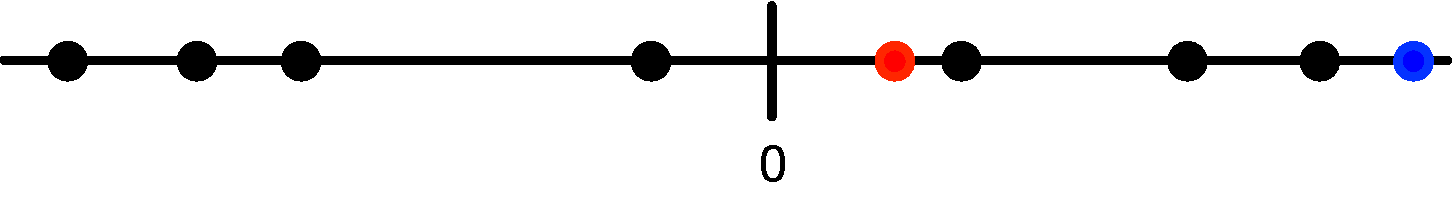
\includegraphics[width=1\textwidth]{lectLR/yesNoCases.pdf} 
\end{frame}
%***********************************************************
%\begin{frame}{Examples from our Music Dataset}
%\begin{itemize}
%\item 
%\end{itemize}
%{\tiny
%\begin {table}[H]
%\begin{tabular}{|r|r|r|r|}
%\hline
% Artist Name & Artist Hottness &  Release Name & Song Hottness   \\ \hline \hline
%Kanye West  & Late Registration & 1.08 & 0.88   \\ \hline
%SOGNQWU12A8AE4868F  & Eurythmics & 207 & 0   \\ \hline
%SOZWHVZ12A6D4F90E7  & U2 & 485 & 3   \\ \hline
%SOGOQGE12AB0182907  & The Killers & 284 & 4   \\ \hline
%SONCHNB12AB01849A2  & Wade Ray & 136  & 3   \\ \hline
%
%\end{tabular}
%\end{table}
%}
%\end{frame}
%***********************************************************
\begin{frame}{Why is this a Problem?}
\begin{itemize}
\item Example: A song's duration and loudness, can we predict if the tempo will be $\ge 100$?
	\begin{itemize}
	\item One song might have a really short duration, be really quiet
	\item Another song might be of average duration, and be a little quiet
	\item Linear Regression for \textbf{categorical} data tries map both to $-1$
	\begin{itemize}
	\item Rather than letting first map to arbitrarily large value (like $+10$), a really solid ``yes''
	\item And letting the second map to a smaller value (like $+0.5$) since a less solid ``yes''
	\end{itemize}
	\end{itemize}
\item Answer: logistic regression... will consider next time
	\begin{itemize}
	\item Under topic of ``generalized linear models''
	\item Are a general class of probabilistic models based on LR
	\item Logistic regression will allow more obvious ``yes'' cases to fall far above decision boundary
	\item While obvious ``no'' cases fall far below
	\end{itemize}
\end{itemize}
\end{frame}
%***********************************************************
\begin{frame}{Data not Handled Well by Linear Regression: Categorical}
\begin{columns}
\begin{column}{0.5\textwidth}
     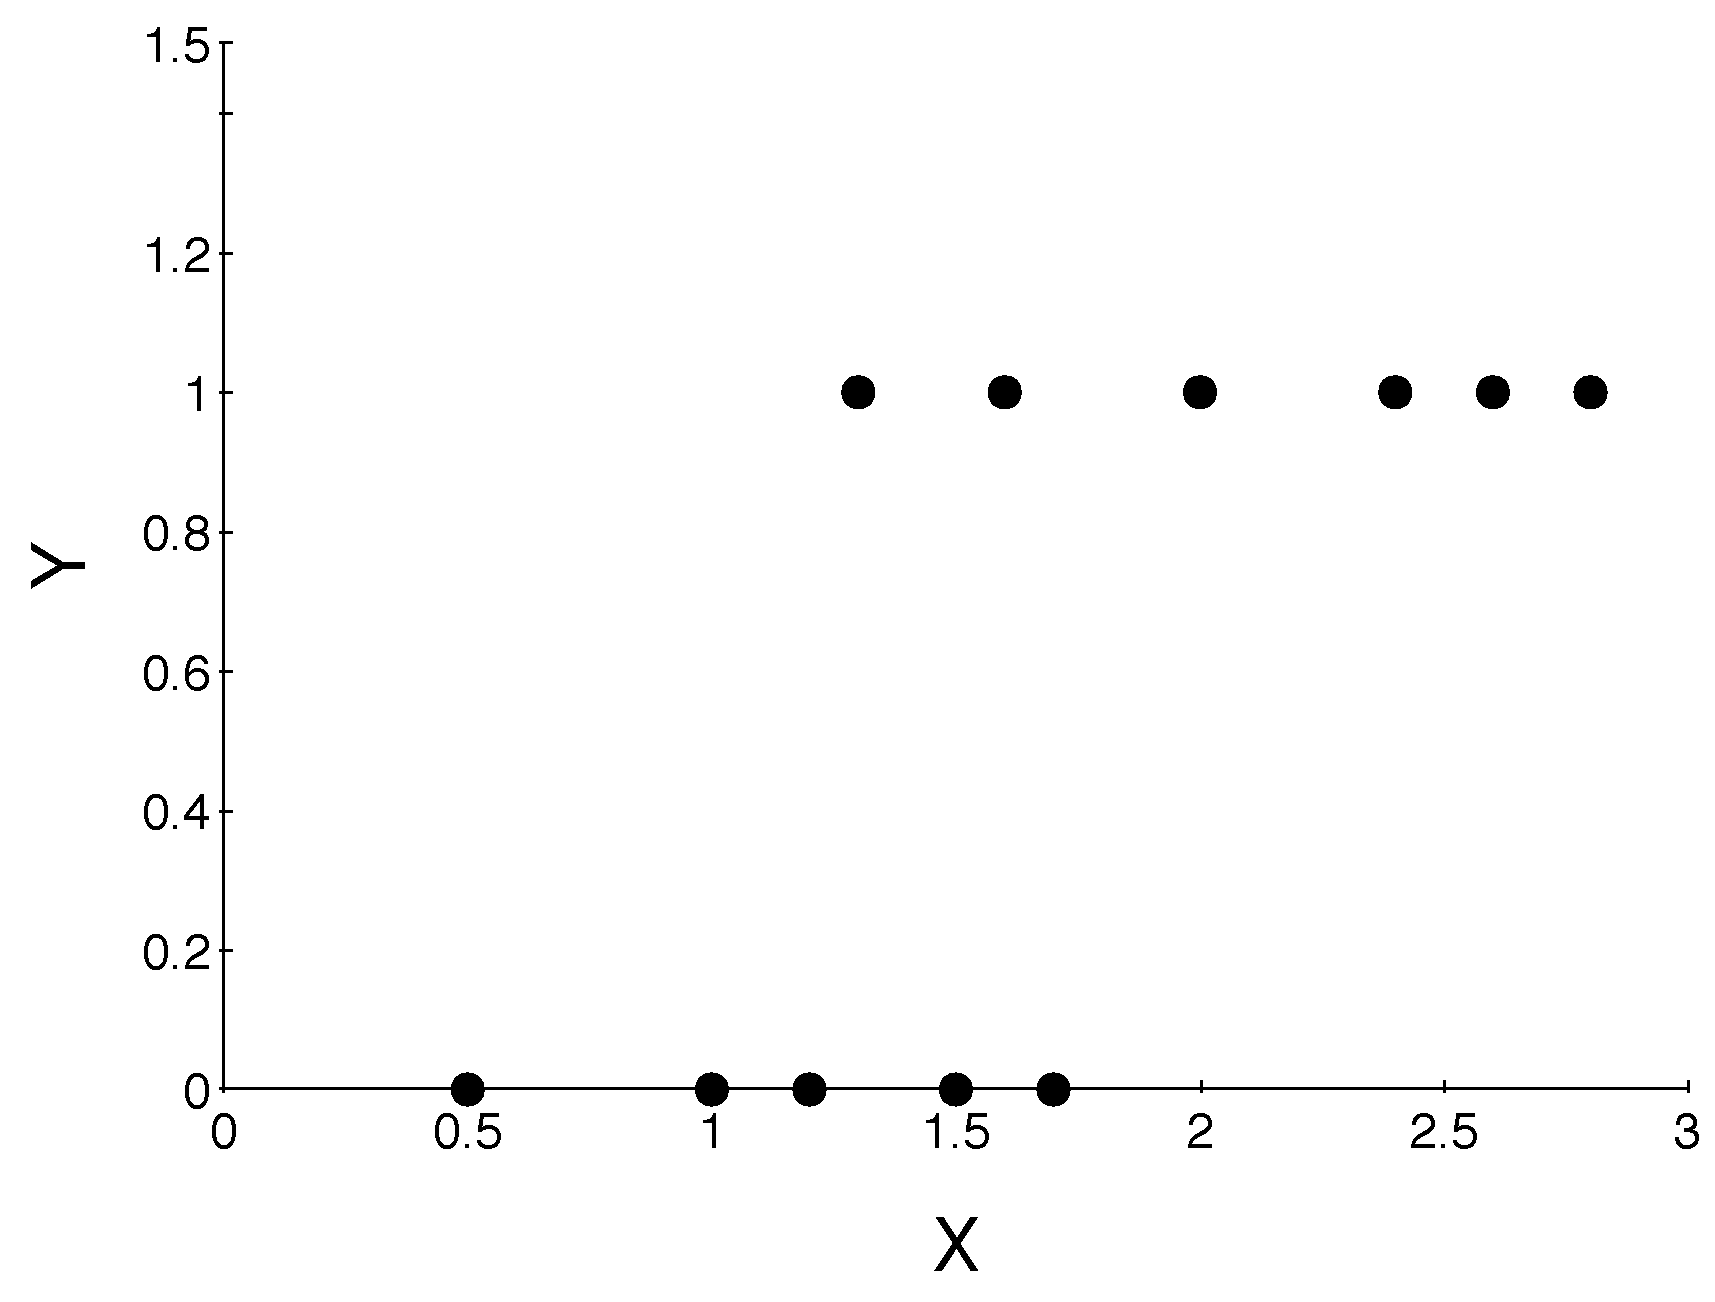
\includegraphics[width=1\textwidth]{lectLR/catData.pdf} 
 \end{column}
\begin{column}{0.5\textwidth}
     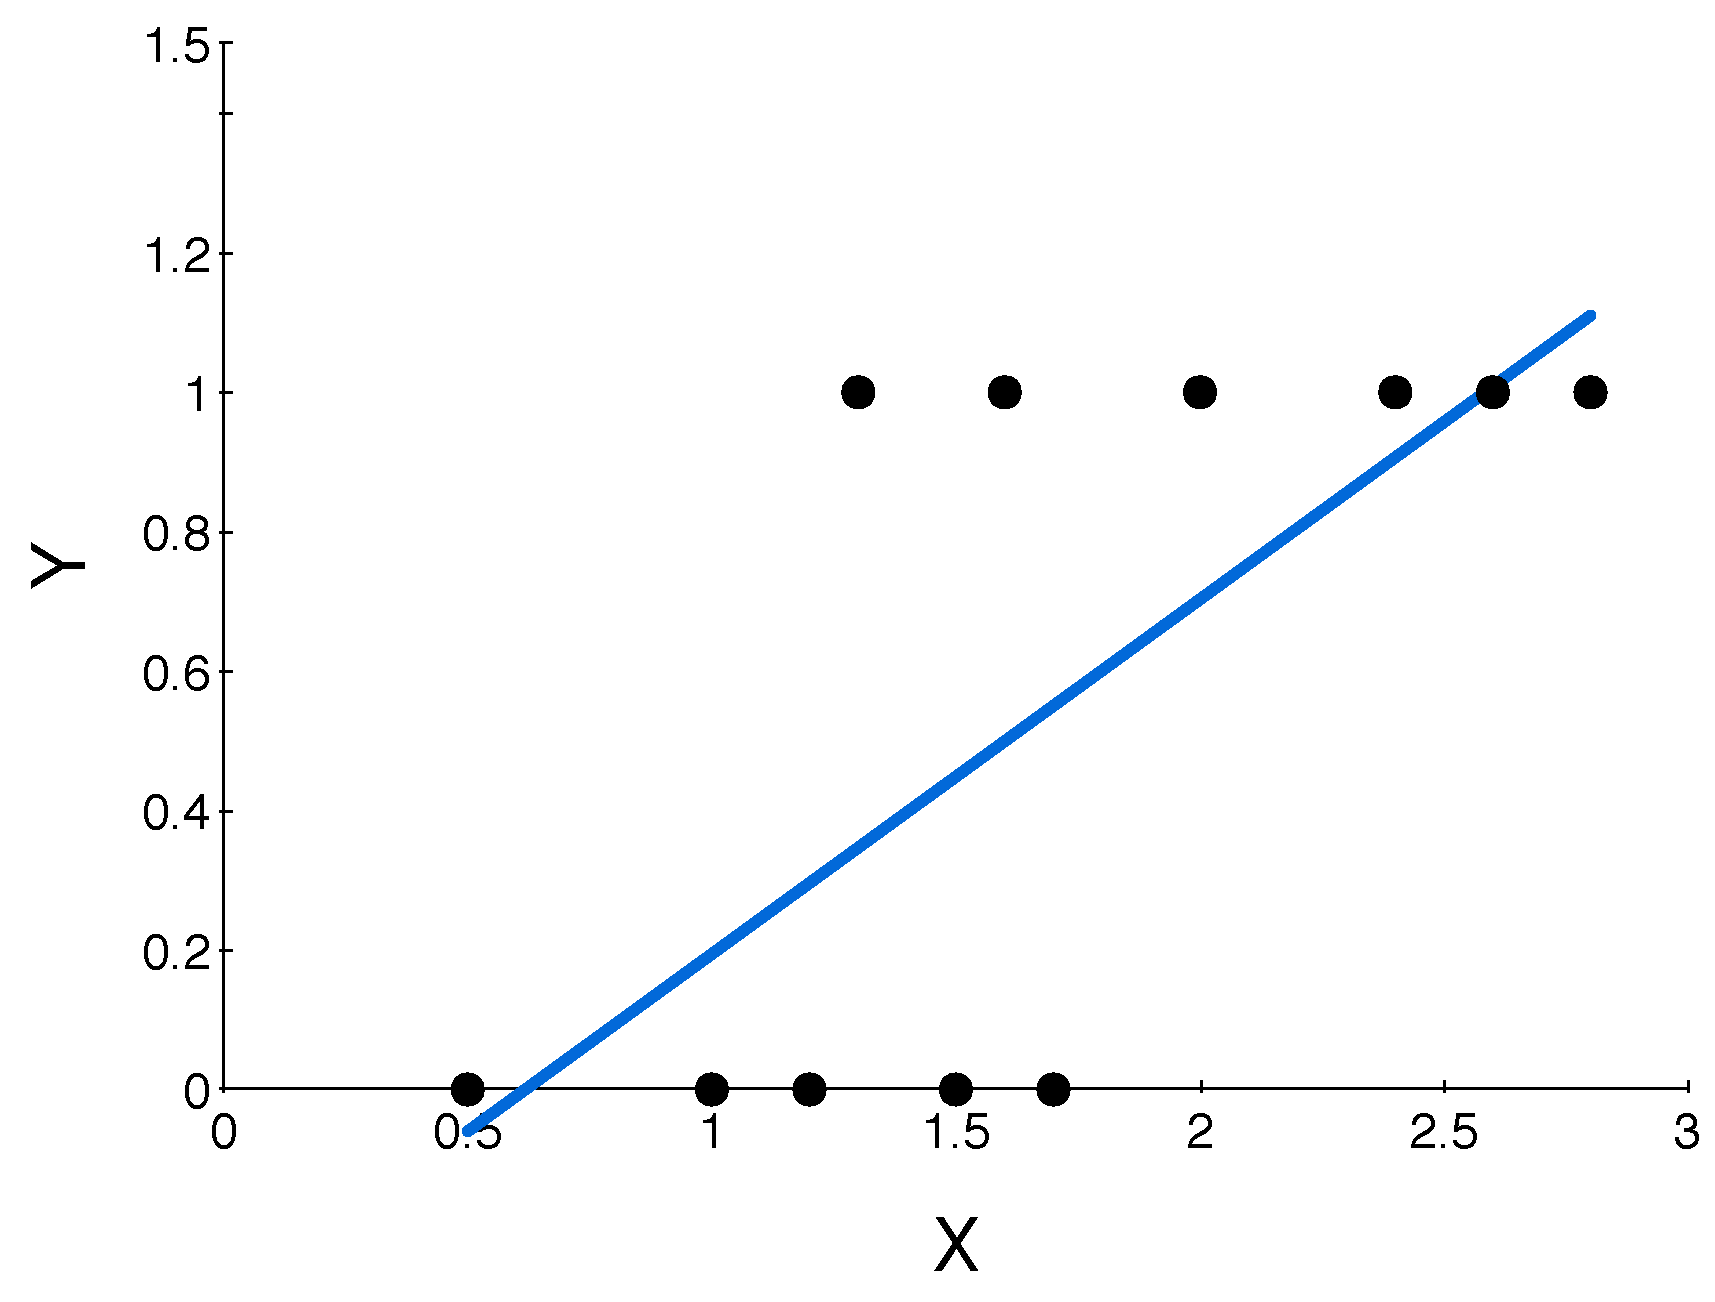
\includegraphics[width=1\textwidth]{lectLR/catDataWithLine.pdf} 
\end{column}
 \end{columns}

\end{frame}

%***********************************************************
\begin{frame}{Data not Handled Well by Linear Regression: Other Non-Linear}
\begin{columns}
\begin{column}{0.5\textwidth}
     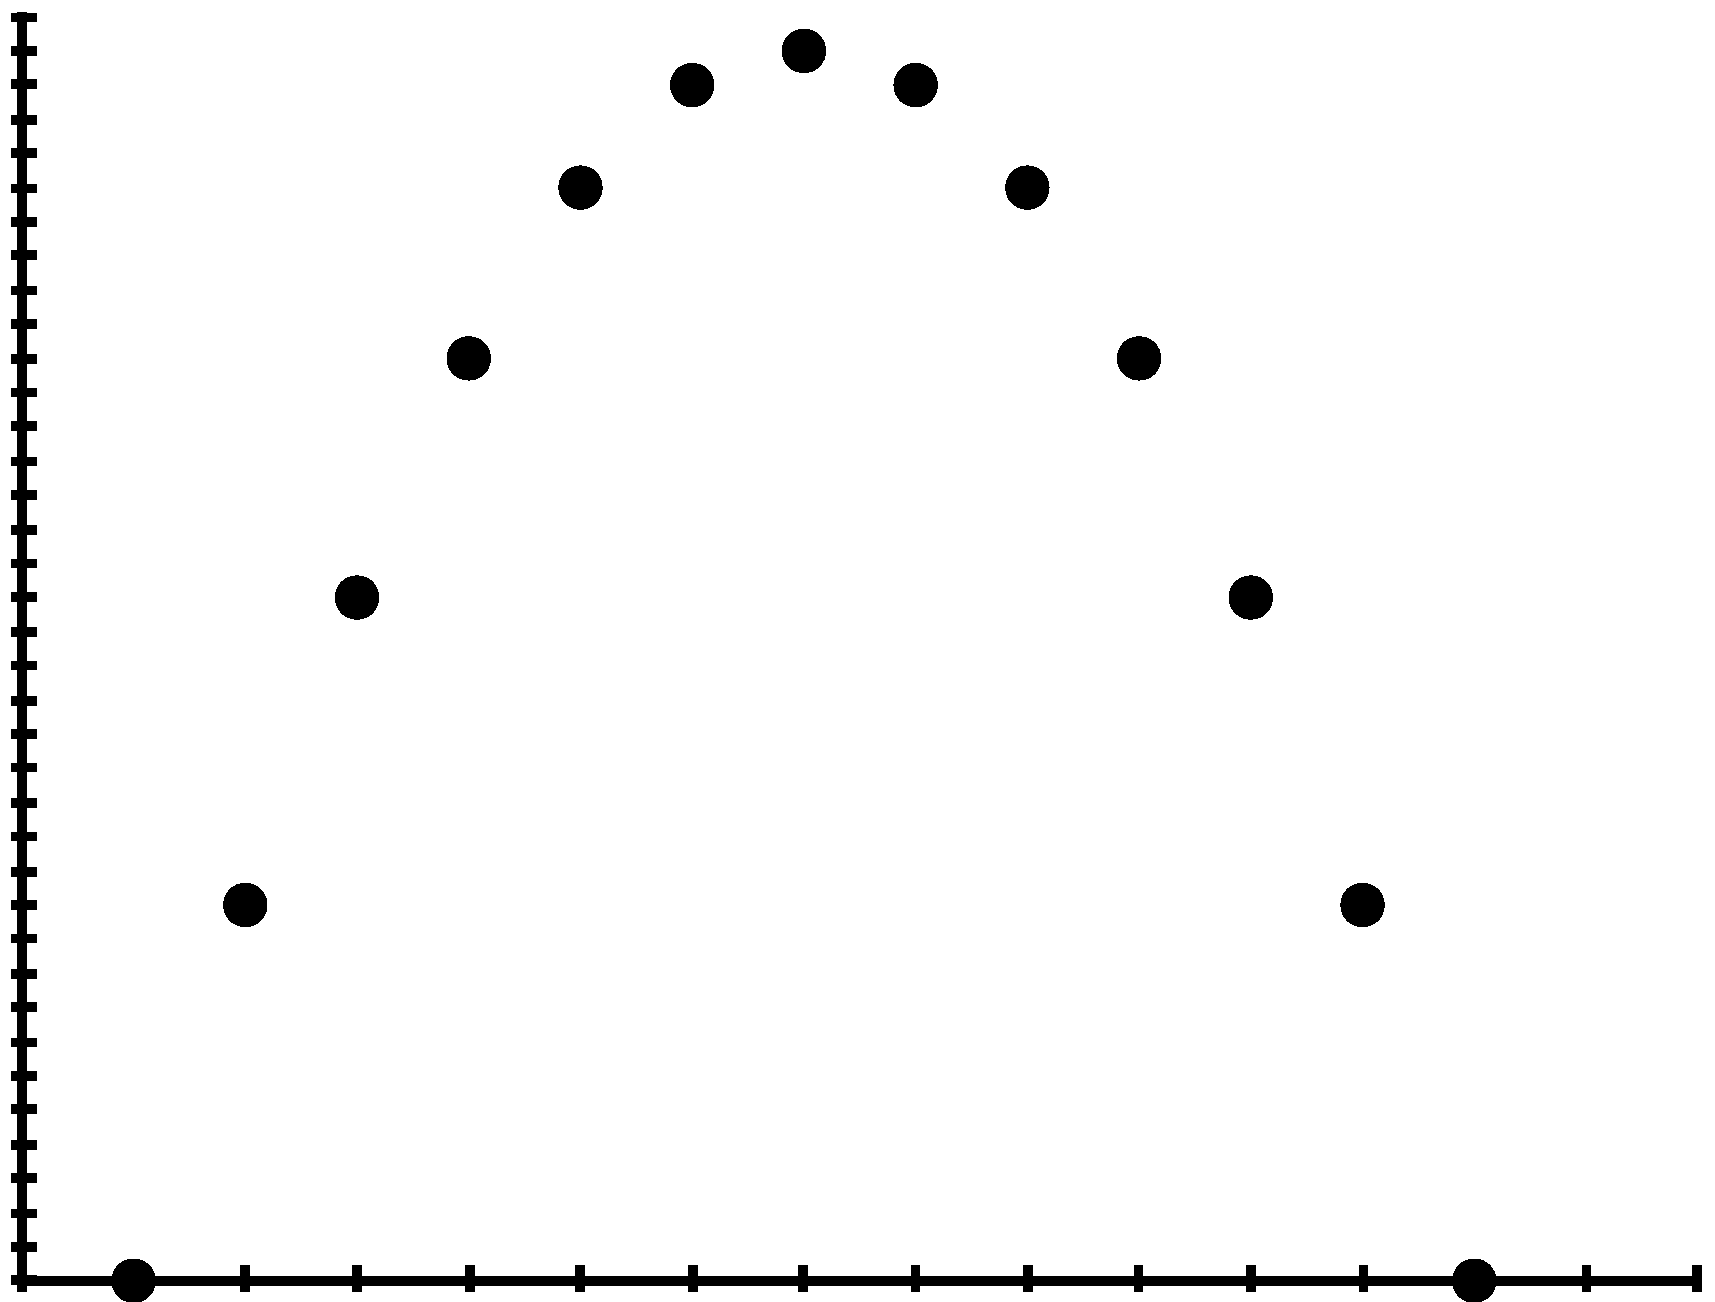
\includegraphics[width=1\textwidth]{lectLR/parabola.pdf} 
 \end{column}
\begin{column}{0.5\textwidth}
     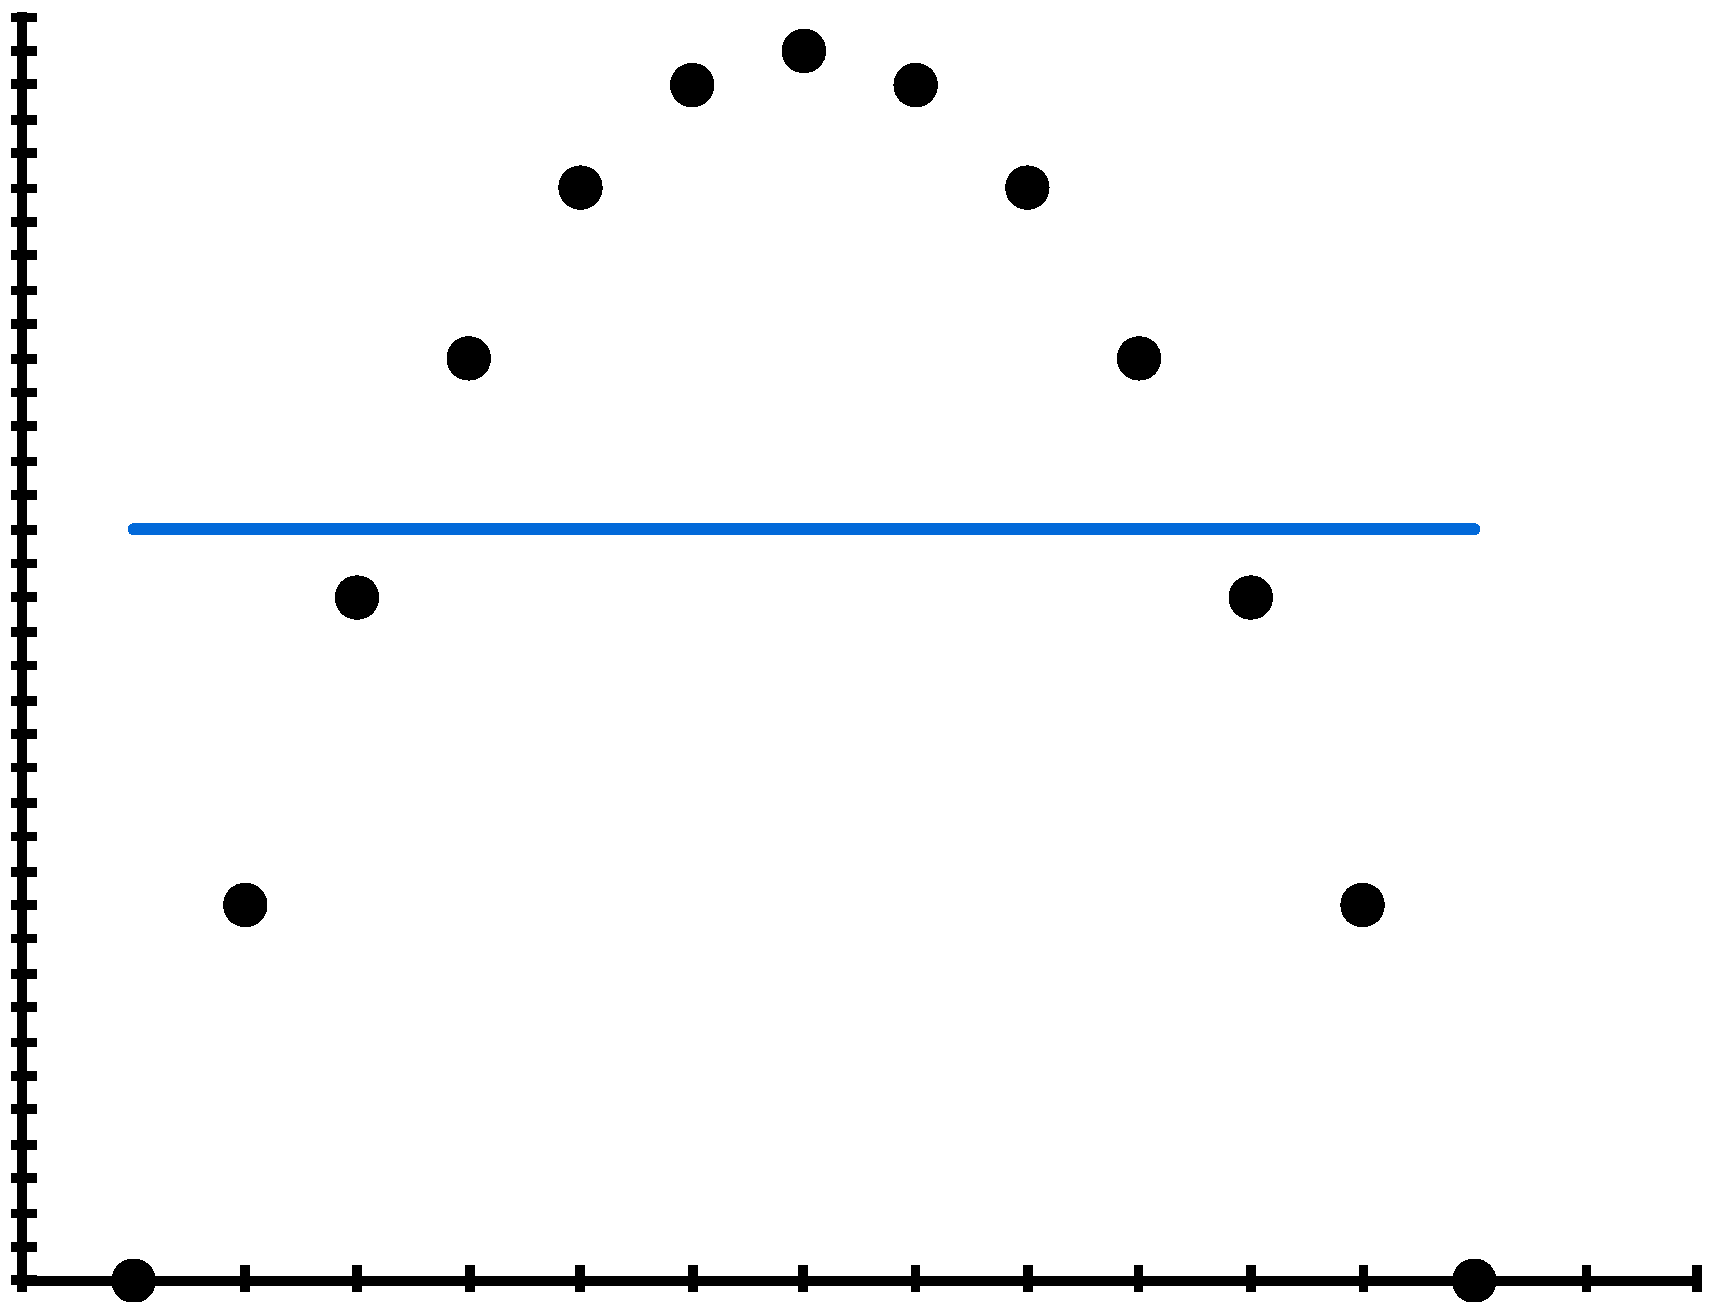
\includegraphics[width=1\textwidth]{lectLR/parabolaWithLine.pdf} 
\end{column}
 \end{columns}

\end{frame}

%***********************************************************
\begin{frame}{Questions?}
\begin{itemize}
	\item What do we know now that we didn't know before?
	\vspace{5 em}
	\item How can we use what we learned today?
\end{itemize}
\end{frame}


\end{document}
